\documentclass{article}
\usepackage{amsmath}
\usepackage{amssymb}
\usepackage{graphicx}
\usepackage{hyperref}
\usepackage[version=4]{mhchem}


\begin{document}
(1992 China Middle School Math Contest) As shown in the figure, in \(\triangle A B C, A B=A C . D\) is a point on \(B C . E\) is a point on \(A D\). \(\angle B E D=2 \angle C E D=\angle A\). Show that \(B D=2 C D\).

Solution:
We draw the circumcircle of \(\triangle A B C\). Extend \(A D\) to meet\\
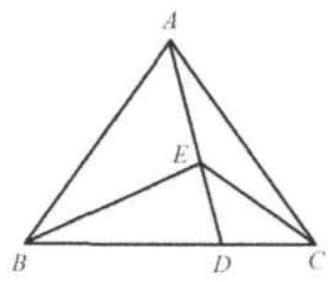
\includegraphics[width=\textwidth]{images/202(2).jpg} the circle at \(F\). Connect \(B F, C F\) (figure 1).\\
Since both angles \(\angle A F B\) and \(\angle A F C\) face the \(\operatorname{arcs}(A B=A C)\) of the same length, \(\angle A F B=\angle A F C=\angle A B C=\theta\).\\
Thus, \(D F\) is the angle bisector of \(\angle B F C\).\\
So by the angle bisector theorem, \(\frac{F B}{F C}=\frac{B D}{C D}\).\\
Now we only need to prove that \(\frac{F B}{F C}=2\) or \(B F=2 C F\).\\
\centering

\includegraphics[width=\textwidth]{images/202.jpg}

We know that in \(\triangle A B C, \angle A+\angle B+\angle C=180^{\circ}\), or \(\angle A+\theta+\theta=180^{\circ}\).

We also know that in \(\triangle E B F, \angle B E F+\angle B F E+\angle E B F=\) \(180^{\circ}\), or \(\angle B E F+\theta+\angle E B F=180^{\circ}\).

Since \(\angle B E D=\angle A, \angle E B F=\theta\).\\
We take the line segment \(B D\) out of the figure and redraw\\
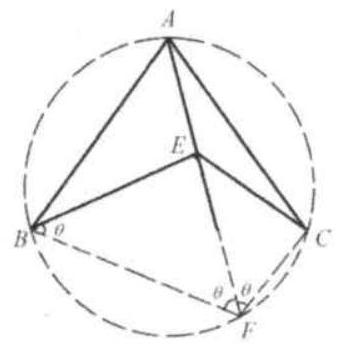
\includegraphics[width=\textwidth]{images/202(1).jpg} the figure (2).

Since \(E B=E F\), we draw \(E G\), the perpendicular bisector of \(B F\).\\
So \(B G=G F, \angle G E B=\angle G E F=C E F=\alpha\) (figure 3).\\
Since \(\angle G E F=\angle C E F=\alpha, E F=E F, \angle E F G=\angle E F C=\theta\),\\
\(\triangle E F G \cong \triangle E F C\). So \(G F=C F\).\\
So we proved that \(B F=2 C F\) and we are done.\\
\centering
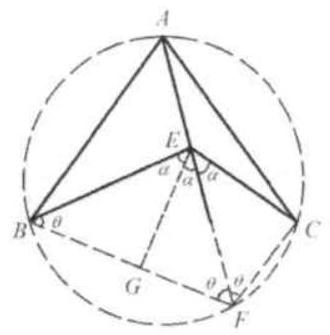
\includegraphics[width=\textwidth]{images/202(3).jpg}



\end{document}
